\documentclass[specification,annotation,times]{itmo-student-thesis}

%% Опции пакета:
%% - specification - если есть, генерируется задание, иначе не генерируется
%% - annotation - если есть, генерируется аннотация, иначе не генерируется
%% - times - делает все шрифтом Times New Roman, собирается с помощью xelatex
%% - pscyr - делает все шрифтом Times New Roman, требует пакета pscyr.

%% Делает запятую в формулах более интеллектуальной, например:
%% $1,5x$ будет читаться как полтора икса, а не один запятая пять иксов.
%% Однако если написать $1, 5x$, то все будет как прежде.
\usepackage{icomma}

%% Данные пакеты необязательны к использованию в бакалаврских/магистерских
%% Они нужны для иллюстративных целей
%% Начало
\usepackage{tikz}
\usetikzlibrary{arrows}
\usepackage{filecontents}

%% Указываем файл с библиографией.
\addbibresource{master-thesis.bib}

\begin{document}

\studygroup{M4239}
\title{Поддержка функций высших порядков в языке KPHP}
\author{Немченко Евгений}{Немченко Е.}
\supervisor{Шалыто Анатолий Абрамович}{Шалыто А.А.}{проф., д.т.н.}{главный научный сотрудник Университета ИТМО}
\publishyear{2019}
%% Дата выдачи задания. Можно не указывать, тогда надо будет заполнить от руки.
\startdate{01}{сентября}{2017}
%% Срок сдачи студентом работы. Можно не указывать, тогда надо будет заполнить от руки.
\finishdate{31}{мая}{2019}
%% Дата защиты. Можно не указывать, тогда надо будет заполнить от руки.
\defencedate{10}{июня}{2019}

%\addconsultant{Белашенков Н.Р.}{канд. физ.-мат. наук, без звания}
%\addconsultant{Беззубик В.В.}{без степени, без звания}

\secretary{Павлова О.Н.}

%% Задание
%%% Техническое задание и исходные данные к работе
\technicalspec{Требуется поддержать функции высших порядков в языке KPHP. Поддержать замыкание переменных, неявное замыкание внутри классов и авто замыкание при передаче методов классов в другие функции. Добавить возможность сохранения, передачи, возврата из других функций анонимных функций. Добавить возможность типизиривать встроенные функции принимающие другие функции, используя зависимые типы. Разрешить сохранять анонимные функции в поля классов. Проверить кодовую базу VK на наличие ошибок при передаче лямбда-функций во встроенные функции. Провести сравнительный анализ с другими решениями. }

%%% Содержание выпускной квалификационной работы (перечень подлежащих разработке вопросов)
\plannedcontents{
\begin{enumerate}
	\item Изучение предметной области и существующих решений;
	\item Исследование возможных решений поставленной задачи;
	\item Разработка синтаксиса и реализация кодогенерации в языке KPHP;
	\item Сравнение производительности с другими решениями.
\end{enumerate}
}

%%% Исходные материалы и пособия 
\plannedsources{\begin{enumerate}
    \item предыдущая версия языка KPHP, который использовался в компании ООО <<В Контакте>>;
    \item спецификация анонимных функций, представленная в виде документации к языку PHP;
    \item Alfred V. Aho, Monica S. Lam, Ravi Sethi, and Jeffrey D. Ullman. 2006. Compilers: Principles, Techniques, and Tools (2nd Edition). Addison-Wesley Longman Publishing Co., Inc., Boston, MA, USA.
\end{enumerate}}

%%% Цель исследования
\researchaim{Изучить и разработать подходящее решение для поддержки функций высших порядков в языке KPHP.}

%%% Задачи, решаемые в ВКР
\researchtargets{\begin{enumerate}
    \item создание синтаксиса для описания функций высших порядков в KPHP;
    \item поддержка анонимных функций и их типизация;
    \item генерация кода и сравнительный анализ производительности.
\end{enumerate}}

%%% Использование современных пакетов компьютерных программ и технологий
\addadvancedsoftware{C++}{\ref{sec2:runtime_principle}}
\addadvancedsoftware{GCC}{\ref{sec:template_functions}}
\addadvancedsoftware{PHP}{\ref{sec:actuality}}

%%% Краткая характеристика полученных результатов 
\researchsummary{Данная работа нашла применение в компании ООО <<В Контакте>>. Улучшила качество написанного кода и помогла найти ошибки, допущенные при написании сайта. Также была разработана система обнаружения ошибок, связанных с типизацией лямбда-функций, которые не способны найти другие решение в данной области.}

%%% Гранты, полученные при выполнении работы 
\researchfunding{}

%%% Наличие публикаций и выступлений на конференциях по теме выпускной работы
\researchpublications{
\textit{Публикации:}
\begin{refsection}
\nocite{nemchenko-vestnik,nemchenko-isledovatel}
\printannobibliography
\end{refsection}
\textit{Конференции:}
\begin{refsection}
\nocite{nemchenko-kmu}
\printannobibliography
\end{refsection}
}

%% Эта команда генерирует титульный лист и аннотацию.
\maketitle{Магистр}

%% Оглавление
\tableofcontents
%-*-coding: utf-8-*-
\startprefacepage
<<ВКонтакте>> - социальная сеть, большая часть которой разрабатывается на языке PHP, начиная с 2006 года.
В 2013 году суточная посещаемость ВКонтакте достигла почти 50 млн. пользователей \cite{kphp-vk-2013} и социальная сеть столкнулась с проблемой обработки большого числа запросов.
Было принято решение о разработке нового инструмента для ускорения и уменьшения потребления памяти занимаемой работой PHP скрипта.
KPHP был разработан для ускорения, написанного кода, который транслировал PHP код в C++.
По факту не было поддержки ООП и функционального стиля, но этого было достаточно, чтобы перевести сайт на KPHP, ускорив тем самым загрузку страниц почти в два раза.

С того времени было написано много нового кода, внутренняя инфраструктура развивалось и возникала необходимость в поддержке нового синтаксиса и соответствующей функциональности.
В современном мире функциональное программирование занимает важную роль, благодаря которому увеличивается производительность программистов, а код становится более выразительным \cite{fp-matters}.
Хорошо структурированные программы легки в написании, отлаживании, чтении и предоставляют набор модулей, которые с без труда могут быть переиспользованы, что в свою очередь уменьшает стоимость доработок в будущем. Функции высших порядков и анонимные функции улучшают модульность программ.
В KPHP существовала возможность передачи указателей на функции во встроенные методы, но нельзя было передавать указатели в произвольные функции и сохранять их в переменные.
Из-за этого приходилось писать громоздкий код, который было сложно поддерживать.

В связи с тем, что не было возможности в KPHP задания типа принимаемой функции приходилось обобщать возвращаемый тип таких функций как \verb|array_map| до типа-суммы, что ухудшало производительность и увеличивало потребление памяти.
С появлением в языке инстансов классов пропала возможность использования стандартных функций с массивом экземпляров классов, т. к. генерировать все возможные типы-суммы из пользовательских классов и примитивных типов не представляется возможным из-за их количества.
Данные проблемы будут описаны подробнее в первой главе.

Далее будет подробнее рассмотрена поставленная задача и подходы необходимые для успешной поддержки функций высших порядков и анонимных функций в языке KPHP.
Будет представлен созданный синтаксис для типизации внутренних функций высших порядков.
Увидим, что потеря типизации ухудшает статический анализ и увеличивает количество ошибок в коде.
Рассмотрим как можно реализовать данную функциональность и не потерять в производительности и потреблении памяти.
Также будет приведен сравнительный анализ других инструментов позволяющих решать эту задачу, например HHVM \cite{hhvm} и PHP7.0 \cite{php7}, а также возможности для дальнейшего развития.

%-*-coding: utf-8-*-

\chapter{Постановка задачи}
Язык KPHP уже существует более пяти лет за это время образовалась достаточно большая кодовая база.
Сейчас в проекте более 60000 строк кода и почти 30000 строк в файлах, содержащих тесты к нему, по результатам запуска \verb|sloccount| \cite{sloccount}. Так как мы решили, что должны добавить поддержку функций высших порядков и анонимных функций, важно было придумать лаконичное решение, вписывающиеся в текущую архитектуру.

В данной работе нам предстоит придумать, как организовать логику передачи анонимных функций и сохранения их в переменные. KPHP - типизированный язык для данной задачи необходимо придумать соответствующую логику, вписывающуюся в имеющуюся архитектуру. Продумать как будут анонимные функции транслироваться в C++ код и что они будут представлять из себя. Каждый вызов анонимной функции транслировать в соответствующий код вызывающий нужную функцию, который корректно обрабатывает все входные данные и захватит нужное окружение.

Для передачи лямбд, методов и других функций в качестве аргументов можно использовать мономорфизацию, которая отлично вписывается в текущую архитектуру, но вот для записи в одно и тоже поле класса разных объектов лямбда функций будет сложнее. Для этого необходимо разработать интерфейсы и соответствующий синтаксис для возможности задания функционального типа в коде и сохранение в него различных объектов, которые можно вызывать без потери производительности, которые в свою очередь будут автоматически наследоваться от соответствующего интерфейса. 

Нужно продумать как поддержать ссылочную семантику для интерфейсов. Добавить возможность задания классов, которые реализуют тот или иной интерфейс, продумать дизайн для создания наследования интерфейсов друг от друга. Сделать статический анализ на корректность классов, реализующих какие-либо интерфейсы. Поддержать возможность проверки на подтип \verb|instanceof| и сделать возможным понижающие приведение. Также нужно научиться поддерживать состояние для различных переменных, экземпляром какого из подтипа она может являться, чтобы автоматически производить понижающее приведение где это необходимо - это должно значительно упростить использование интерфейсов разработчиками.

Для уменьшения ошибок при написании анонимных функций с захватом внешних переменных разработать синтаксис, который будет ограничивать переменные на запись, добавляя им семантику константных переменных. Зачастую разработчики не ожидают поведения, предоставляемого языков PHP, когда они пытаются изменить захваченные переменные, а если им нужно будет поменять, то нужно будет всего лишь скопировать в другую переменную, чтобы наверняка понимать, что захваченные аргументы не меняют своих значений.

Нужно продумать новый синтаксис для типизации встроенных в язык функций таких как \verb|array_map|, \verb|array_reduce| и другие. Все они принимают анонимную функцию в качестве аргумента, типы аргументов которой зависят от передаваемых параметров встроенной функции. Разработав систему задания типов для анонимных функций, нужно понять, как внедрить это в язык KPHP, для корректного сопоставления с типами во всех местах использования.

\section{Термины и понятия}
\textbf{Трансляция} -- перевод из одного языка программирования в другой с целью ускорения и уменьшения потребления памяти.

\textbf{Лямбда функция} -- функция, которая не имеет уникального идентификатора и обычно создаются в месте использования.

\textbf{Анонимная функция} -- лямбда функция.

\textbf{Функция высших порядков} -- либо принимает другую функцию как аргумент, либо возвращает созданную в теле функцию.

\textbf{Захваченная переменная} -- переменная, которая была сохранена и продолжает существовать внутри лямбда функции.

\textbf{Ссылочная семантика} -- когда любое присвоение объектов в другие переменные копирует только ссылку на него.

\textbf{Понижающее приведение} -- преобразование переменной, ссылающийся на базовый класс, к одному из производных классов.

\textbf{Встроенные функции} -- функции которые написаны на C++, тело которых скрыто для разработчиков на языке KPHP, однако они имеют возможность вызывать их.

\textbf{Типизация} -- процесс сопоставления различных переменных с соответствующими типами, а также возвращаемых значений функций.

\textbf{Проверка на подтип} -- процесс в результате которого получается булевское значение истинность которого показывает является ли соответствующая переменная данным подтипом.

\textbf{Инстанс} -- один из экземпляров конкретного класса.

\textbf{Мономорфизация} -- техника, которая заключается в порождении мономорфного экземпляра для каждого случая использования полиморфной функции или типа.

\textbf{Примитивный тип} -- такой тип, встроенный в язык KPHP, который может представлять из себя один из типов: целых чисел, вещественных чисел, значений из булева множества, строк, а также массивов.

\textbf{Тип-сумма} -- тип, построенный как дизъюнктное объедение исходных типов.

\textbf{Рантайм} -- среда выполнения или такое окружение, которое необходимо для выполнения программы. В KPHP - это отдельная подключаемая библиотека.

\textbf{CFG} -- граф потока управления, множество всех возможных путей исполнения программы, представленное в виде графa.

\textbf{AST} -- абстрактное синтаксическое дерево, представляет из себя дерево, каждая вершина которого обозначает конструкцию, встречающуюся в исходном коде.

\textbf{Манглирование}

\section{Актуальность}
\label{sec:actuality}
На текущий момент существует несколько способов решения поставленной задачи. Один из простых вариант, который можно рассмотреть -- это отказ от использования KPHP в пользу других языков программирования. 
Радикально менять язык программирования будет достаточно большой и трудоемкой задачей, которая вовлечет за собой огромные денежные затраты со стороны компании и вряд ли оправдает свою стоимость. 
В кодовой базе насчитывается более двух миллионов строк кода, написанных на языке KPHP (совместимым с PHP).
Даже если нанять 100 программистов, которые каждый рабочий день будут переписывать по 100 строчек кода, то у них уйдет на это почти пять месяцев. За это время конечно же появится новый код, а еще нужно будет интегрировать в текущую архитектуру и исправить все допущенные ошибки - на это тоже уйдет достаточно много времени.
Из-за трудоемкости и неоправданной дороговизне мы не будем рассматривать данное решение в дальнейшем.

Посмотрим, что еще мы можем предпринять в данной ситуации. 
Так как код написан на PHP, то кажется разумным решением его и запускать с помощью интерпретатора. 
Этот подход имеет право на существование, но как мы увидим в следующих главах он также имеет множество недостатков.
Например, KPHP анализирует написанный код, что позволяет находить массу ошибок, допущенных программистами.
Также в KPHP существует дополнительные возможности, совместимые с языком PHP, для применения дополнительных ограничений на переменные и проверка их до момента запуска.
Основным преимуществом конечно же является скорость работы, которая позволяет уменьшить количество дорогостоящих серверов, что в свою очередь влечет снижение расходов компании на содержание и закупку новых.

Следующим кандидатом может выступать язык Hack и его виртуальная машина HHVM, разработанные в компании facebook.
Данный язык является диалектом PHP, который позволяет совмещать в себе динамическую и статическую типизацию.
У него есть несколько недостатков, из-за которых его использование не подходит компании:

\begin{enumerate}
\item Он не совместим с языком PHP, что вызывает некоторые сложности в его использовании, как минимум нужно будет исправить много кода, а также мы лишимся возможности использовать стандартные средства для статического анализа, так как все они предназначены для PHP;

\item Хоть у него и есть JIT, данный язык с его окружением по-прежнему на многих тестах медленнее KPHP, что будет показано далее, что приведет нас к покупке дополнительных серверов и колоссальным затратам на их поддержку;

\item Нужно переделать существующую инфраструктура для развёртывания необходимого программного обеспечения на сервера, что тоже займет не мало времени, в том числе возникнут дополнительные проблемы и спецэффекты о которых мы сейчас даже не можем предположить.
\end{enumerate}

Из приведенных аргументов выше мы понимаем, что переход на другие языки, даже очень близкие к KPHP невозможен на текущем этапе развития компании, то давайте взглянем на несколько примеров, которые могут заменить использование лямбд и функций высших порядков в языке.
Посмотрим, что происходит, если у нас отсутствует возможность сохранять анонимные функции в переменные:
\begin{lstlisting}[caption={Пример кода без анонимных функций},label={without_lambda}]
function debug_for_foo($x) {
  var_dump("in foo: value of x: {$x}");
}

function foo() {
  $x = get_new_x();
  debug_for_foo($x);

  $y = calc_value($x);
  debug_for_foo($y);
}
\end{lstlisting}

В листинге \ref{without_lambda} видно, что небольшой дублирующийся код мы вместо того, чтобы вынести локально в переменную, содержащую анонимную функцию, и тут же его вызывать, вынуждены определять в отдельной функции.
Также на этом примере наглядно продемонстрирована проблема того, что при вынесении всех таких мелких вспомогательных функций мы будем вынуждены манглировать их имена специальным образом, если их тело будет отличаться в разных функциях, что приводят к загромождению кода и загрязнению глобального пространства имен функций.
С использованием лямбд мы могли бы переписать его следующим образом, что несомненно улучшает читаемость кода и уменьшает затраченное время на написание его:
\begin{lstlisting}
function foo() {
  $debug = function($x) { var_dump("in foo: value of x: {$x}"); };
  $x = get_new_x();
  $debug($x);

  $y = calc_value($x);
  $debug($y);
}
\end{lstlisting}

Теперь посмотрим, как можно обойти проблему отсутствия функций высших порядков, с помощью определения нескольких функций, которые будут вызывать другие функции:
\begin{lstlisting}[caption={Пример кода без функций высших порядков},label={without_getting_lambda}]
function debug_result_of_call($result) {
  var_dump("in function foo: value of x: {$x}");
}

function get_x_y_from_net() {
	return [get_x_from_server(), get_y_from_server()];
}

function get_sum($x, $y) {
    return $x + $y;
}

function debug_result_of_call_sum() {
	list($x, $y) = get_x_y_from_net();
	debug_result_of_call(get_sum($x, $y));
}

function get_sub($x, $y) {
    return $x - $y;
}

function debug_result_of_call_sub() {
	list($x, $y) = get_x_y_from_net();
	debug_result_of_call(get_sub($x, $y));
}

function debug_combinations_of_x_y() {
	debug_result_of_call_sum();
	debug_result_of_call_sub();
}
\end{lstlisting}

В листинге \ref{without_getting_lambda} отображены явные недостатки отсутствия функций высших порядков.
Так как мы хотим максимально избавиться от дублирования кода, мы вынуждены все общие части выносить в отдельные функции.
На этом примере также показана необходимость создания временных имен, для того, чтобы вызывать разные функции и чем больше будет таких примеров, тем сильнее разрастется код ненужными сущностями, которые ухудшают читаемость и склоны к ошибкам, допускаемыми при копировании похожих частей кода.
Давайте взглянем как надо было бы решать данную проблему используя функции высших порядков:
\begin{lstlisting}
function debug_result(callable $get_result) {
	list(x, y) = [get_x_from_server(), get_y_from_server()];
	var_dump("in function foo: value of x: ".$get_result($x));
}

function debug_combinations_of_x_y() {
	debug_result(function ($x, $y) { return $x + $y; });
	debug_result(function ($x, $y) { return $x - $y; });
}
\end{lstlisting}

Простота и изящность - так можно охарактеризовать, приведенный код выше.
Данный листинг показывает, что писать на языке без лямбда-функций и функций высших порядков довольно таки сложно, а допустить ошибку в коде становится намного легче.
Давайте взглянем какие еще сложности у нас возникают в текущей момент.
На данном этапе у нас нет синтаксиса, для спецификации типов аргументов лямбда функций и типа возвращаемого значения, поэтому, считается, что все они возвращают некоторый тип-суммы примитивных типов.
Что в свою очередь приводит к тому, что мы не можем их использовать с экземплярами классов, например:
\begin{lstlisting}
class MyClass { public $x = 10; }

$arr = [new MyClass(), new MyClass];
$xs = array_map(function($m) { return $m->x; }, $arr);
\end{lstlisting}

Этот пример отображает невозможность написать такой код, так как принимаемое значение должно иметь примитивный тип, а мы пытаемся передать ему экземпляр класса.
Соответственно все встроенные функции будут запрещены в использовании с классами.
Также использования встроенных функций с лямбда-функциями там, где тип выводится верно, например, с массивом чисел мы получим ухудшения в производительности, из-за обобщения примитивных типов до типа-суммы.


\section{Уточненные требования к работе}
В предыдущей секции мы рассмотрели примеры и убедились в необходимости создания поддержки лямбд и анонимных функций в языке KPHP. Давайте попробуем детализировать этапы, необходимые для совершения данной работы и что нам предстоит реализовать.

Сначала нужно разобраться, а что из себя представляют анонимные функции, прочитать соответствующую спецификацию к языку PHP и выделить основные моменты и детали синтаксиса.
Мы должны будем написать разбор таких функций с дальнейшим построением AST, введя необходимые типы вершин для этого.
Надо решить во что мы будем транслировать создание анонимных функций и как будет происходить вызов, надо не забыть поддержать ссылочную семантику при создании лямбда-функций.
Также стоит определить куда сохранять захваченные переменные в тело лямбда-функции, а после необходим модифицировать ее тело таким образом, чтобы все обращения к захваченным переменным происходили через экземпляр класса лямбда-функции.
Нужно учитывать, что при определении лямбды внутри метода класса, нужно неявно захватывать \verb|$this|, а также позаботиться о том, что все обращения внутри \verb|$this->field_name| были корректно обработаны.

Следующим этапом будет продумывание семантики для захваченных переменных, как говорилось ранее нужно придумать синтаксис, который бы ограничивал, захваченные переменные на запись.
Соответственно стоит ввести аннотацию \verb|@kphp-const| и соответствующие модификаторы во внутренних структурах, позволяющие проверять на изменения данных переменных.
Также соответственно надо разработать инфраструктуру для проверки кода, и выдачи ошибок пользователям о произошедшей модификации переменной, которая помечена данной аннотацией.

Для создания функций высших порядков, необходимо придумать каким образом мы будем передавать туда лямбда функции, так как мы транслируем в типизированный язык, а семантика PHP запрещает перегрузку функций, то необходимо произвести соответствующую мономорфизацию функций, принимающих другие функции.
Соответственно необходимо разработать специальный синтаксис для поддержки шаблонных функций в языке KPHP, которыми смогут пользоваться другие разработчики и по возможности автоматически понимать в каких местах можно аннотировать параметры как шаблонные за них.

Надо разработать новый синтаксис для типизации передаваемых анонимных функций во встроенные функции.
Аннотировать разработанным синтаксисом все существующие стандартные функции.
Поддержать их синтаксический анализ и сохранение нужной метаинформации в вершинах AST дерева.
Внедрить вывод типов для случаев передачи лямбд в стандартные функции.
Поддержать корректную трансляцию таких вызовов, а также рассмотреть, как выводить результирующие типы корректно во всех возможных случаях использования.

Для того чтобы появилась возможность сохранять различные лямбда функции, но имеющие схожую сигнатуру в одну и ту же переменную, надо разработать поддержку интерфейсов в языке.
Для чего необходимо изучить текущую спецификацию их и возможные подводные камни.
Разобрать синтаксис, научиться транслировать их.
Также необходимо разработать генерацию виртуальных методов интерфейсов и проверку на подтип.

\chapterconclusion
В данной главе мы детально познакомились с поставленной задачей.
Разобрали ее актуальность и необходимость реализации.
Привели примеры в каких ситуациях без поддержки данной функциональности у нас не получится должного дальнейшего развития языка.
Сравнили с другими решениями из чего заключили, что принятое решение о разработке именно в языке KPHP данной задачи оправдано.

Также были рассмотрены этапы, необходимые для построения архитектуры и дальнейшего анализа, отражающие сложность и многогранность поставленной перед нами задачи.
В следующих главах остановимся подробнее на каждом этапе и посмотрим какие варианты были бы приемлемы для решения и почему мы остановились именно на таком варианте.
Также будет показано сравнение разработанного решения с аналогами и увидим оправданность справедливость данных подходов.

%-*-coding: utf-8-*-

\chapter{Описание технических аспектов реализации}

\section{Общий принцип работы}

\section{Анонимные функции}
\subsection{Разбор синтаксиса}
\subsection{Вывод типов}
\subsection{Кодогенерация}

\section{Шаблонные функции}

\section{Поддержка интерфейсов}
\subsection{Разбор синтаксиса}
\subsection{Генерация методов}
\subsection{Лямбды как члены классов}

\chapterconclusion

%-*-coding: utf-8-*-

\chapter{Сравнение с другими решениями}
В данной главе будут рассмотрены спроектированные и реализованные решения для поддержки лямбда-функций и функций высших порядков.
Посмотрим как влияют на производительность и память одинаковые конструкции в языках Hack, PHP и KPHP.
Посмотрим какие ошибки стали обнаруживаться при добавление анонимных функций.

\section{Потребление CPU для различных решений}
Давайте рассмотрим время затраченное на различные конструкции.
Начнем с того, сколько времени у нас занимает простое создание лямбда-функций.
Тест представленный в листинге \ref{lst:benchmark-create-simple}, будет в цикле много раз создавать обычную лямбда-функцию, KPHP - не будет оптимизировать простое создание, так как сейчас внутри происходят вызовы функций, находящихся в других единицах трансляции, поэтому тест получится объективными.
\begin{lstlisting}[caption={Бенчмарк создания анонимных функций},label={lst:benchmark-create-simple}]
$n = (int)2e8;
$res = 0;
for ($i = 0; $i < $n; $i++) {
    $f = function($x) { return $x; };
    $res ^= $i;
}
var_dump($res);
\end{lstlisting}

Проделав замер времени работы, получаем следующую картину, показанную на рисунке \ref{fig:benchmark-create-simple}.
Hack представил себя медленнее KPHP всего в 1.3 раза, но эти результаты получились после JIT-а, так например первые 10 запросов к серверу HHVM работали по 12 секунд для теста из листинга \ref{lst:benchmark-create-simple}.
\begin{figure}[H]
    \caption{Сравнение затраченного времени на создание лямбда-функций}
    \label{fig:benchmark-create-simple}
    \centering
    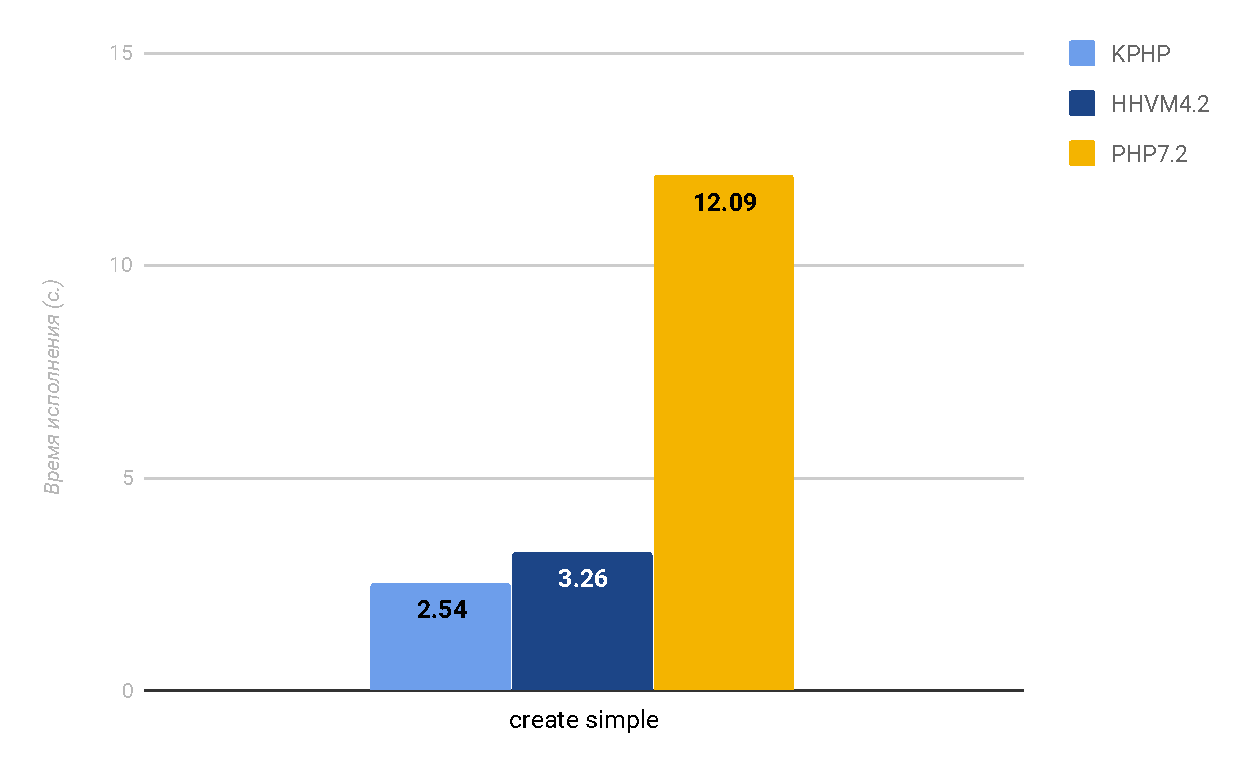
\includegraphics[width=\linewidth]{images/benchmark_create_simple}
\end{figure}

Сравним время которое уходит на вызов созданной лямбда-функции.
Код, который был запущен на всех трех языках представлен в листинге \ref{lst:benchmark-call-simple}.
\begin{lstlisting}[caption={Бенчмарк вызовов анонимных функций},label={lst:benchmark-call-simple}]
$n = (int)2e8;
$res = 0;
$f = function($x) { return $x; };
for ($i = 0; $i < $n; $i++) {
    $res ^= f($i);
}
var_dump($res);
\end{lstlisting}

Результат замеров дал следующие результаты представленные на рисунке \ref{fig:benchmark-call-simple}.
мы видимо как вызов лямбда-функции успешно был встроен в место использования, что привело к нулевым накладным расходам.
\begin{figure}[H]
    \caption{Сравнение затраченного времени на вызов лямбда-функций}
    \label{fig:benchmark-call-simple}
    \centering
    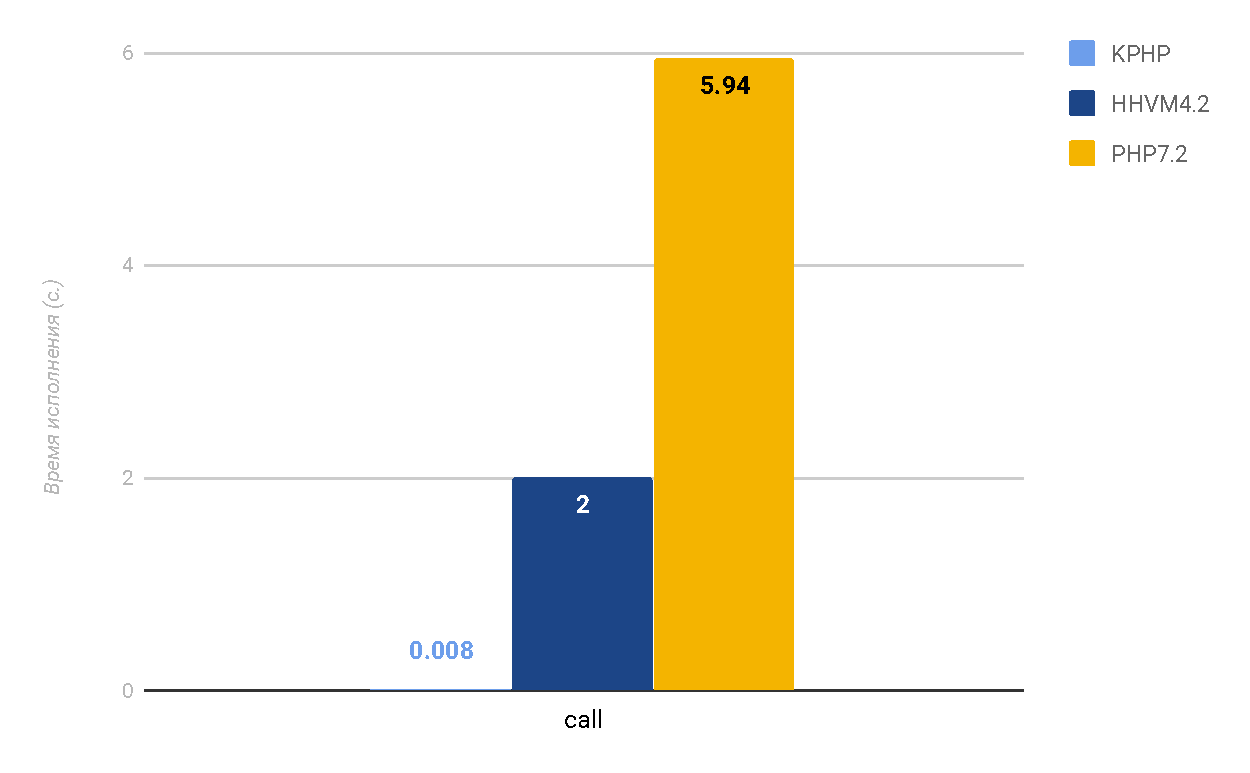
\includegraphics[width=\linewidth]{images/benchmark_call_simple}
\end{figure}

Теперь давайте взглянем на время работы копирования анонимных функций в параметры функций.
Создадим простую лямбда-функцию и будем в цикле ее передавать в другую функцию.
Тест представлен в листинге \ref{lst:benchmark-copy-simple}.
\begin{lstlisting}[caption={Бенчмарк копирования анонимных функций},label={lst:benchmark-copy-simple}]
function foo(callable $f) {}

$n = (int)2e8;
$res = 0;
$f = function($x) { return $x; };
for ($i = 0; $i < $n; $i++) {
    foo($f);
}
var_dump($res);
\end{lstlisting}

На рисунке \ref{fig:benchmark-copy-simple} отчетливо видно, как ссылочная семантика и реализация именно через классы хорошо работает.
У нас получилось дешевым, достаточно скопировать один указатель и увеличить счетчик ссылок, без какой-либо дополнительной мета-информации.
\begin{figure}[H]
    \caption{Сравнение затраченного времени на копирование лямбда-функций}
    \label{fig:benchmark-copy-simple}
    \centering
    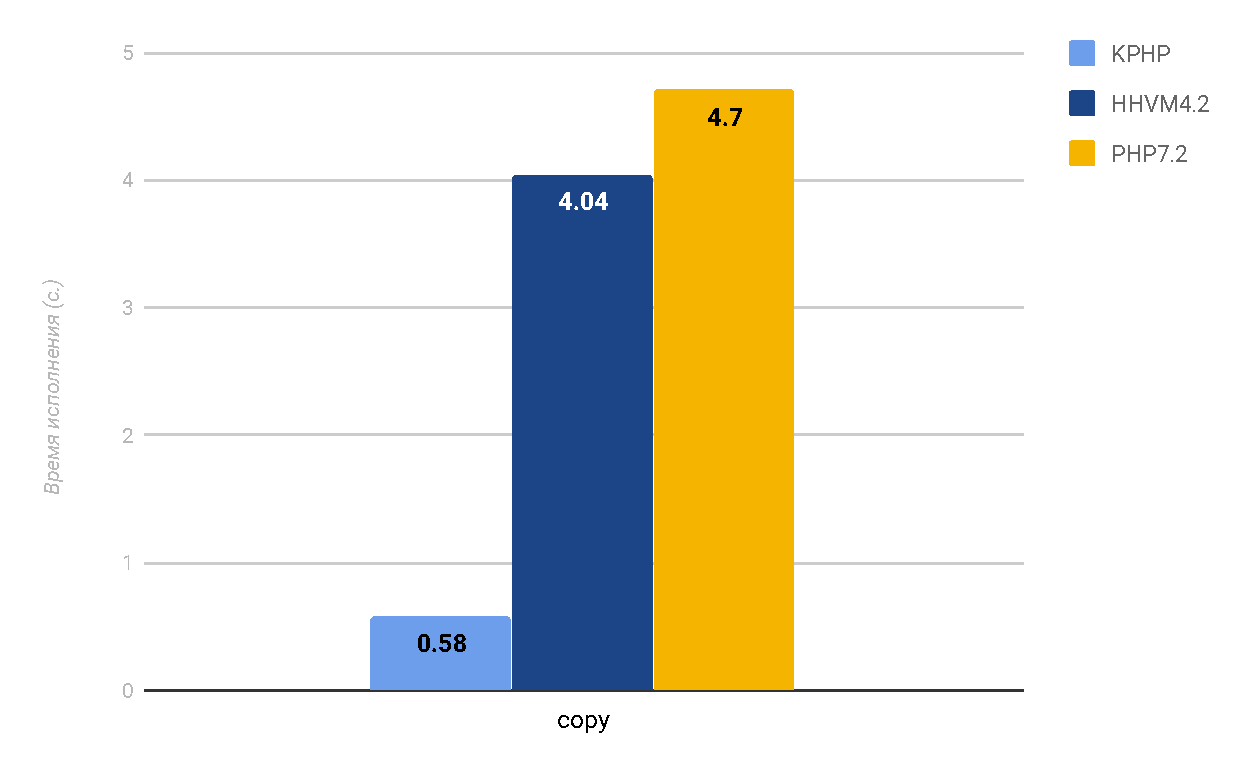
\includegraphics[width=\linewidth]{images/benchmark_copy_simple}
\end{figure}

Также интересно посмотреть на время затраченное при использовании лямбда-функций, которые захватывают переменные из внешнего окружения.
Приведем один общий тест, который сравнивает, сколько времени работает создание и вызов лямбда-функции без захвата переменных и с захватом.
Тест, который запускался на разных языках представлен в листинге \ref{lst:benchmark-create_use_call-simple}, второй запуск был с закомментированной строчкой, которая создают лямбда функции и захватывает переменную.
\begin{lstlisting}[caption={Бенчмарк создания и вызова анонимных функций с захватом},label={lst:benchmark-create_use_call-simple}]
$n = (int)2e8;
$res = 0;
for ($i = 0; $i < $n; $i++) {
    $f = function($x) { return 20 + $x; };
    # $f = function($x) use ($i) { return $i + $x; };
    $res ^= $f($i);
}
var_dump($res);
\end{lstlisting}

На рисунке \ref{fig:benchmark-create_use_call-simple} представлен график сравнения запусков на по очереди заменив использование лямбда-функции с захватом и без.
Диаграмма показывает соотношение времени работы без использования захвата переменных и с использованием.
Можно заметить, что PHP ухудшает производительность почти в 1.5 раза, однако HHVM становится медленнее на 9\%.
В KPHP ничего не меняется, так как компилятор по прежнему справляется встроить лямбда-функцию в место использования и оптимизировать ее.
\begin{figure}[H]
    \caption{Сравнение затраченного времени на создание и вызов анонимных функций с захватом}
    \label{fig:benchmark-create_use_call-simple}
    \centering
    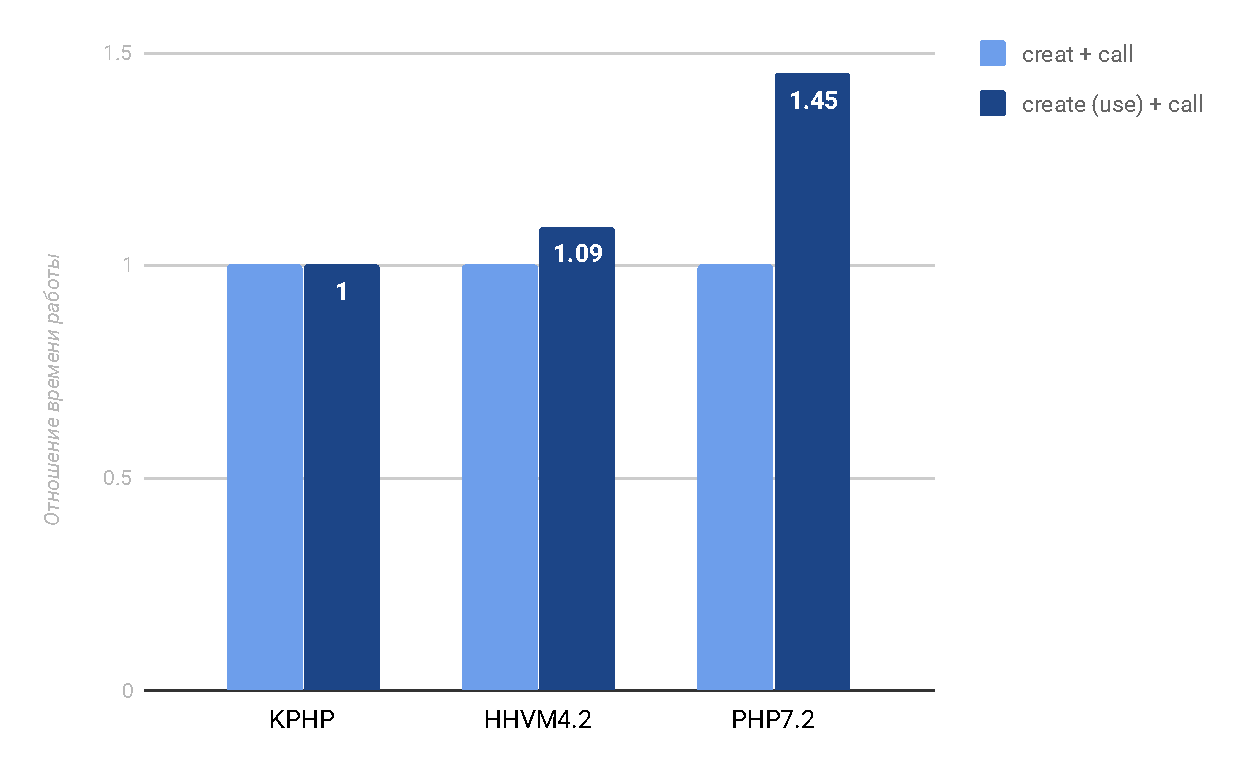
\includegraphics[width=\linewidth]{images/benchmark_create_use_call_simple}
\end{figure}

Давайте посмотрим на время создания интерфейсов.
Было проведено сравнение, в котором в цикле создавались обычные классы и классы которые реализуют интерфейсы.
Сравнение показало, что в PHP работает в 1.5 раза дольше, а Hack медленнее на целых 18\% процентов.
Также было выявлено, что в PHP и в HHVM создание классов с интерфейсами и без интерфейсов не отличается по времени,
однако в KPHP создание классов с интерфейсами работает на 7-8\% дольше.
Запустив программу вместе с \verb|perf|\cit{perf}, было выявлено, что это происходит из-за виртуальных вызовов функций для подсчета ссылок и освобождения памяти.
Так как в случае интерфейсов эти функции не могут быть девиртуализованны\cite{devirtualization}, то встраивание происходит не так глубоко и оптимизитатор работает хуже, что мы и видим при запуске тестов.

Также было проведено сравнение времени работы вызова виртуальных функций.
С помощью этого механизма будут реализован механизм сохранения разных лямбда-функций в одну переменную.
Результаты оказались такими, что сейчас в KPHP сделано совсем не оптимальным способом работа с интерфейсными методами, так как там при каждом вызове в худшем случае может происходить \verb|n| вызовов \verb|dynamic_cast|, где \verb|n| - это количество классов, реализовавших данный интерфейс.
Данное решение можно достаточно легко соптимизировать, заменив подряд идущие проверки на \verb|switch| по \verb|typeid|\cite{fast-dynamic-cast}, однако сейчас это не требуется.
Тесты показали, что сейчас вызов виртуального метода работает в два раза дольше чем у Hack и всего лишь на 18\% процентов быстрее PHP.
Но в при добавлении возможности сохранять лямбда-функции в одну переменную, конечно же данное решение будет ускорено в разы.


\section{Сравнения использованной памяти}
тут посмотрим кто сколько жрет памяти.

\section{Улучшение качества кода и уменьшение ошибок}
Расскажу историю про usort и друзей.
Про более хороший вывод типов.

\chapterconclusion
Здесь мы сравнили.
Убедились, что наше решение работает в разы лучше аналогов.
Также потребляет меньше памяти.
Находит баги и вообще все супер круто.
% -*-coding: utf-8-*-

\startconclusionpage
В настоящей работе были разработаны лямбда-функции, а также функции высших порядков в языке KPHP.
Был добавлена концепция шаблонных функций, которая позволяет производить мономорфизацию в случае вызова с экземплярами разных классов.
Также был разработан специальный синтаксис для аннотирования встроенных функций, позволяющих проверять типы и правильно типизировать параметры и возвращаемое значение лямбда-функции, а также результата встроенных функций.
В рамках данной работы были поддержаны интерфейсы для возможности сохранения разных анонимных функций в одну переменную, сейчас данное решение немного многословно, но в будущем будет не сложно, базируясь на данных разработках, поддержать полноценную возможность сохранения лямбда-функций.

В данной работе мы рассмотрели устройство компилятора и рантайма языка KPHP.
Было показано, как лаконично встроить текущее решение в существующую инфраструктуру.
Было проведено сравнение реализации предложенного подхода с имеющимся аналогами такими как PHP7.2 и HHVM4.2.
Данное сравнение показала, что проделанная работа не накладывает дополнительных накладных расходов, а также, что превосходит другие решение в несколько раз по времени работы.
Мы увидели, что благодаря данной разработке KPHP стал находить ошибки в коде связанные с типизацией лямбда-функций, передаваемых во встроенные функции с чем не справляется ни одно из решений на данный момент.

Данная работа была успешно внедрена и используется сейчас в компании ООО <<В Контакте>>.
Сейчас в кодовой базе насчитывается около 742 анонимных функций, 61 лямбда-функций захватывающих какие-либо переменный.
Также уже написано 55 функций высших порядков.
Были найдены и исправлены ошибки связанные с типизацией лямбда-функций.

Таким образом данная разработка нашла свое применение.
Благодаря достигнутым результатам программисты в компании смогли использовать анонимные функции повсеместно, что доказывает количество их использования с момента поддержки.
Также добавление интерфейсов в язык открывает новые горизонты развития языка KPHP и позволяет писать более понятный и простой код разработчикам сайта.

\printmainbibliography

               
\end{document}

